
\documentclass[journal]{IEEEtran}
\usepackage{blindtext}
\usepackage{graphicx}

\ifCLASSINFOpdf

\else

\fi

\hyphenation{Techno-logy sphe-rical}


\begin{document}

\title{Solar Tracking Improvement using LDR Array}

\author{Achmadi and Purwadi Agus Darwito}

\maketitle


\begin{abstract}

In free energy subject, collecting energy from natural sources is the basic.
This sources such as sun, wind, waterfall, or biological materials.
One of main objective of free energy research is how to increase effeciency and effectiveness.
Thus, finding new optimum energy collection method become popular research subject.
In this work, we introduce a method that suppose to be easy and cheap that can optimize sun energy collecting method.
This method using only LDR (Light Dependent Resistor) that commonly found on the market with low prices.
By arrange some LDR, we can get sun estimation of polar angle and azimuthal angle.
Using output from this sensor array we can get better solar tracking result that can used to optimize sun energy collecting process.\cite{sensor_array}
\end{abstract}

\begin{IEEEkeywords}
LDR Array, Polar Coordinates, Solar Tracking
\end{IEEEkeywords}

\IEEEpeerreviewmaketitle



\section{Introduction}
Sun sensor are widely used for orientation measurement in solar power plants.\cite{sun_sensor_1},\cite{sun_sensor_2}
The traditional approach in the design of sun sensors is to tile flat detectors, which generate electrical current as the sunlight reaches them through an upper window. One can then calculate the incident angle of the light ray by processing the outputs of detectors.\cite{old_sensor_1}-\cite{old_sensor_4}
However, sun position estimation commonly limited if the traditional method used.
Sun position represented by angles commonly only available in one direction only.

A LDR sensor has a limited detection capability.
LDR sensor only detect sun position only in one point.
To increase detection capability then multiple LDR sensor is used.
These multiple LDR sensor arranged in an array.
To approach spherical position of the sun, this sensor array build in a spherical construction.


\subsection{Design}
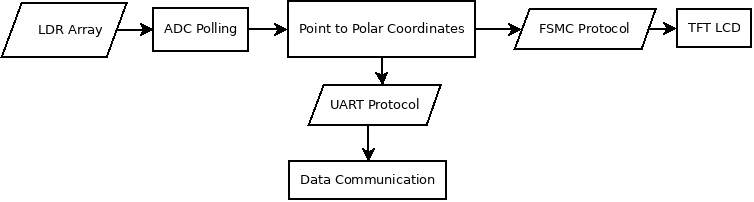
\includegraphics[width=250pt]{skema}\\
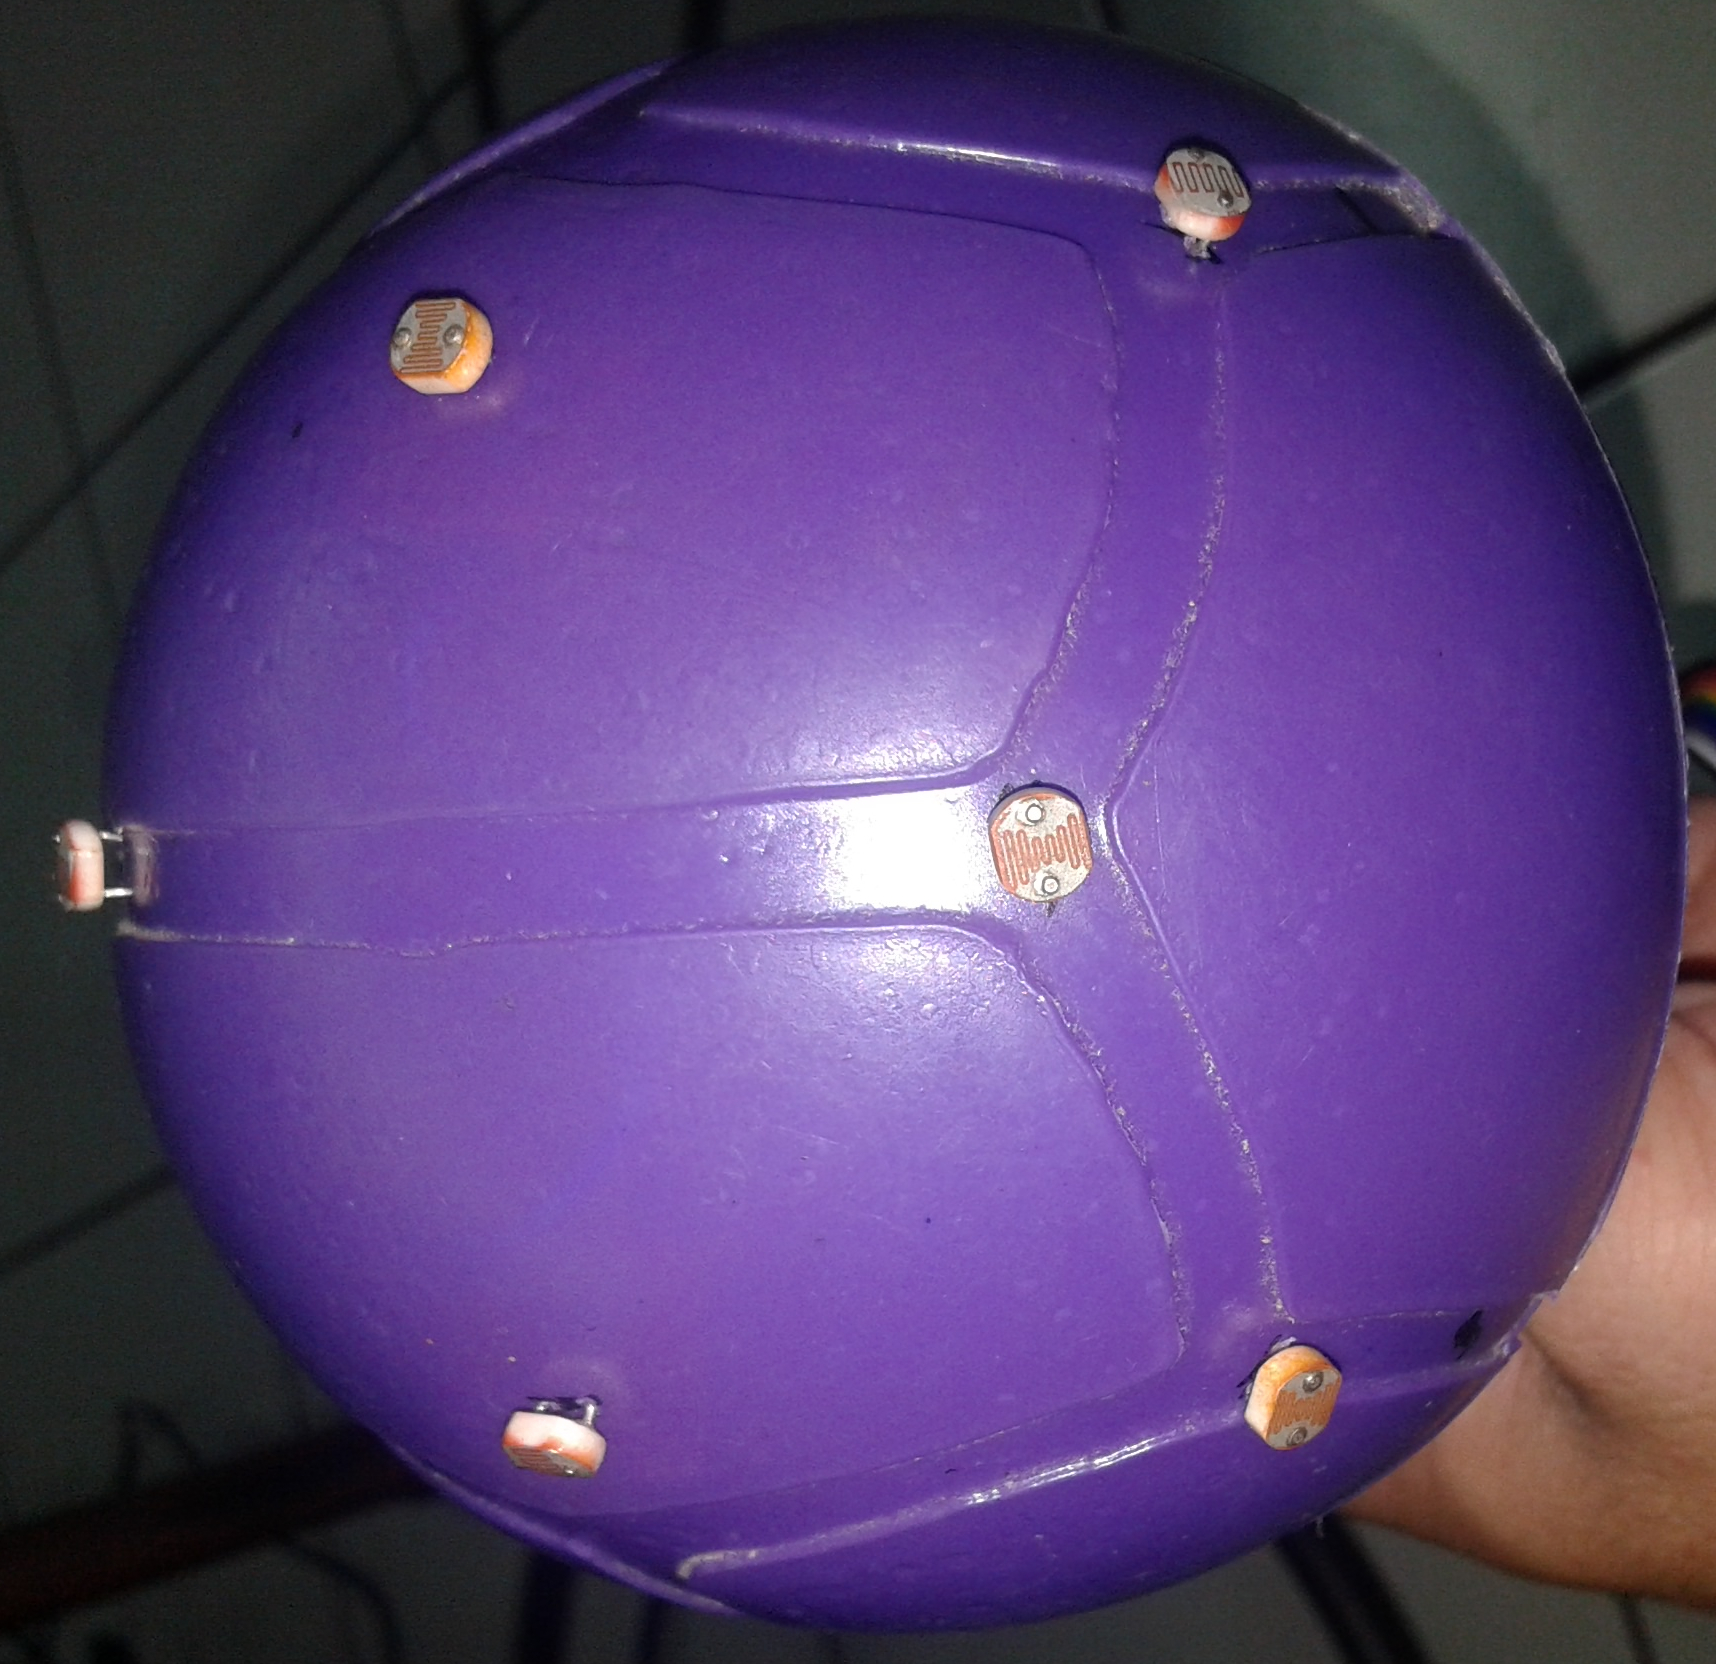
\includegraphics[width=100pt]{sensorball}
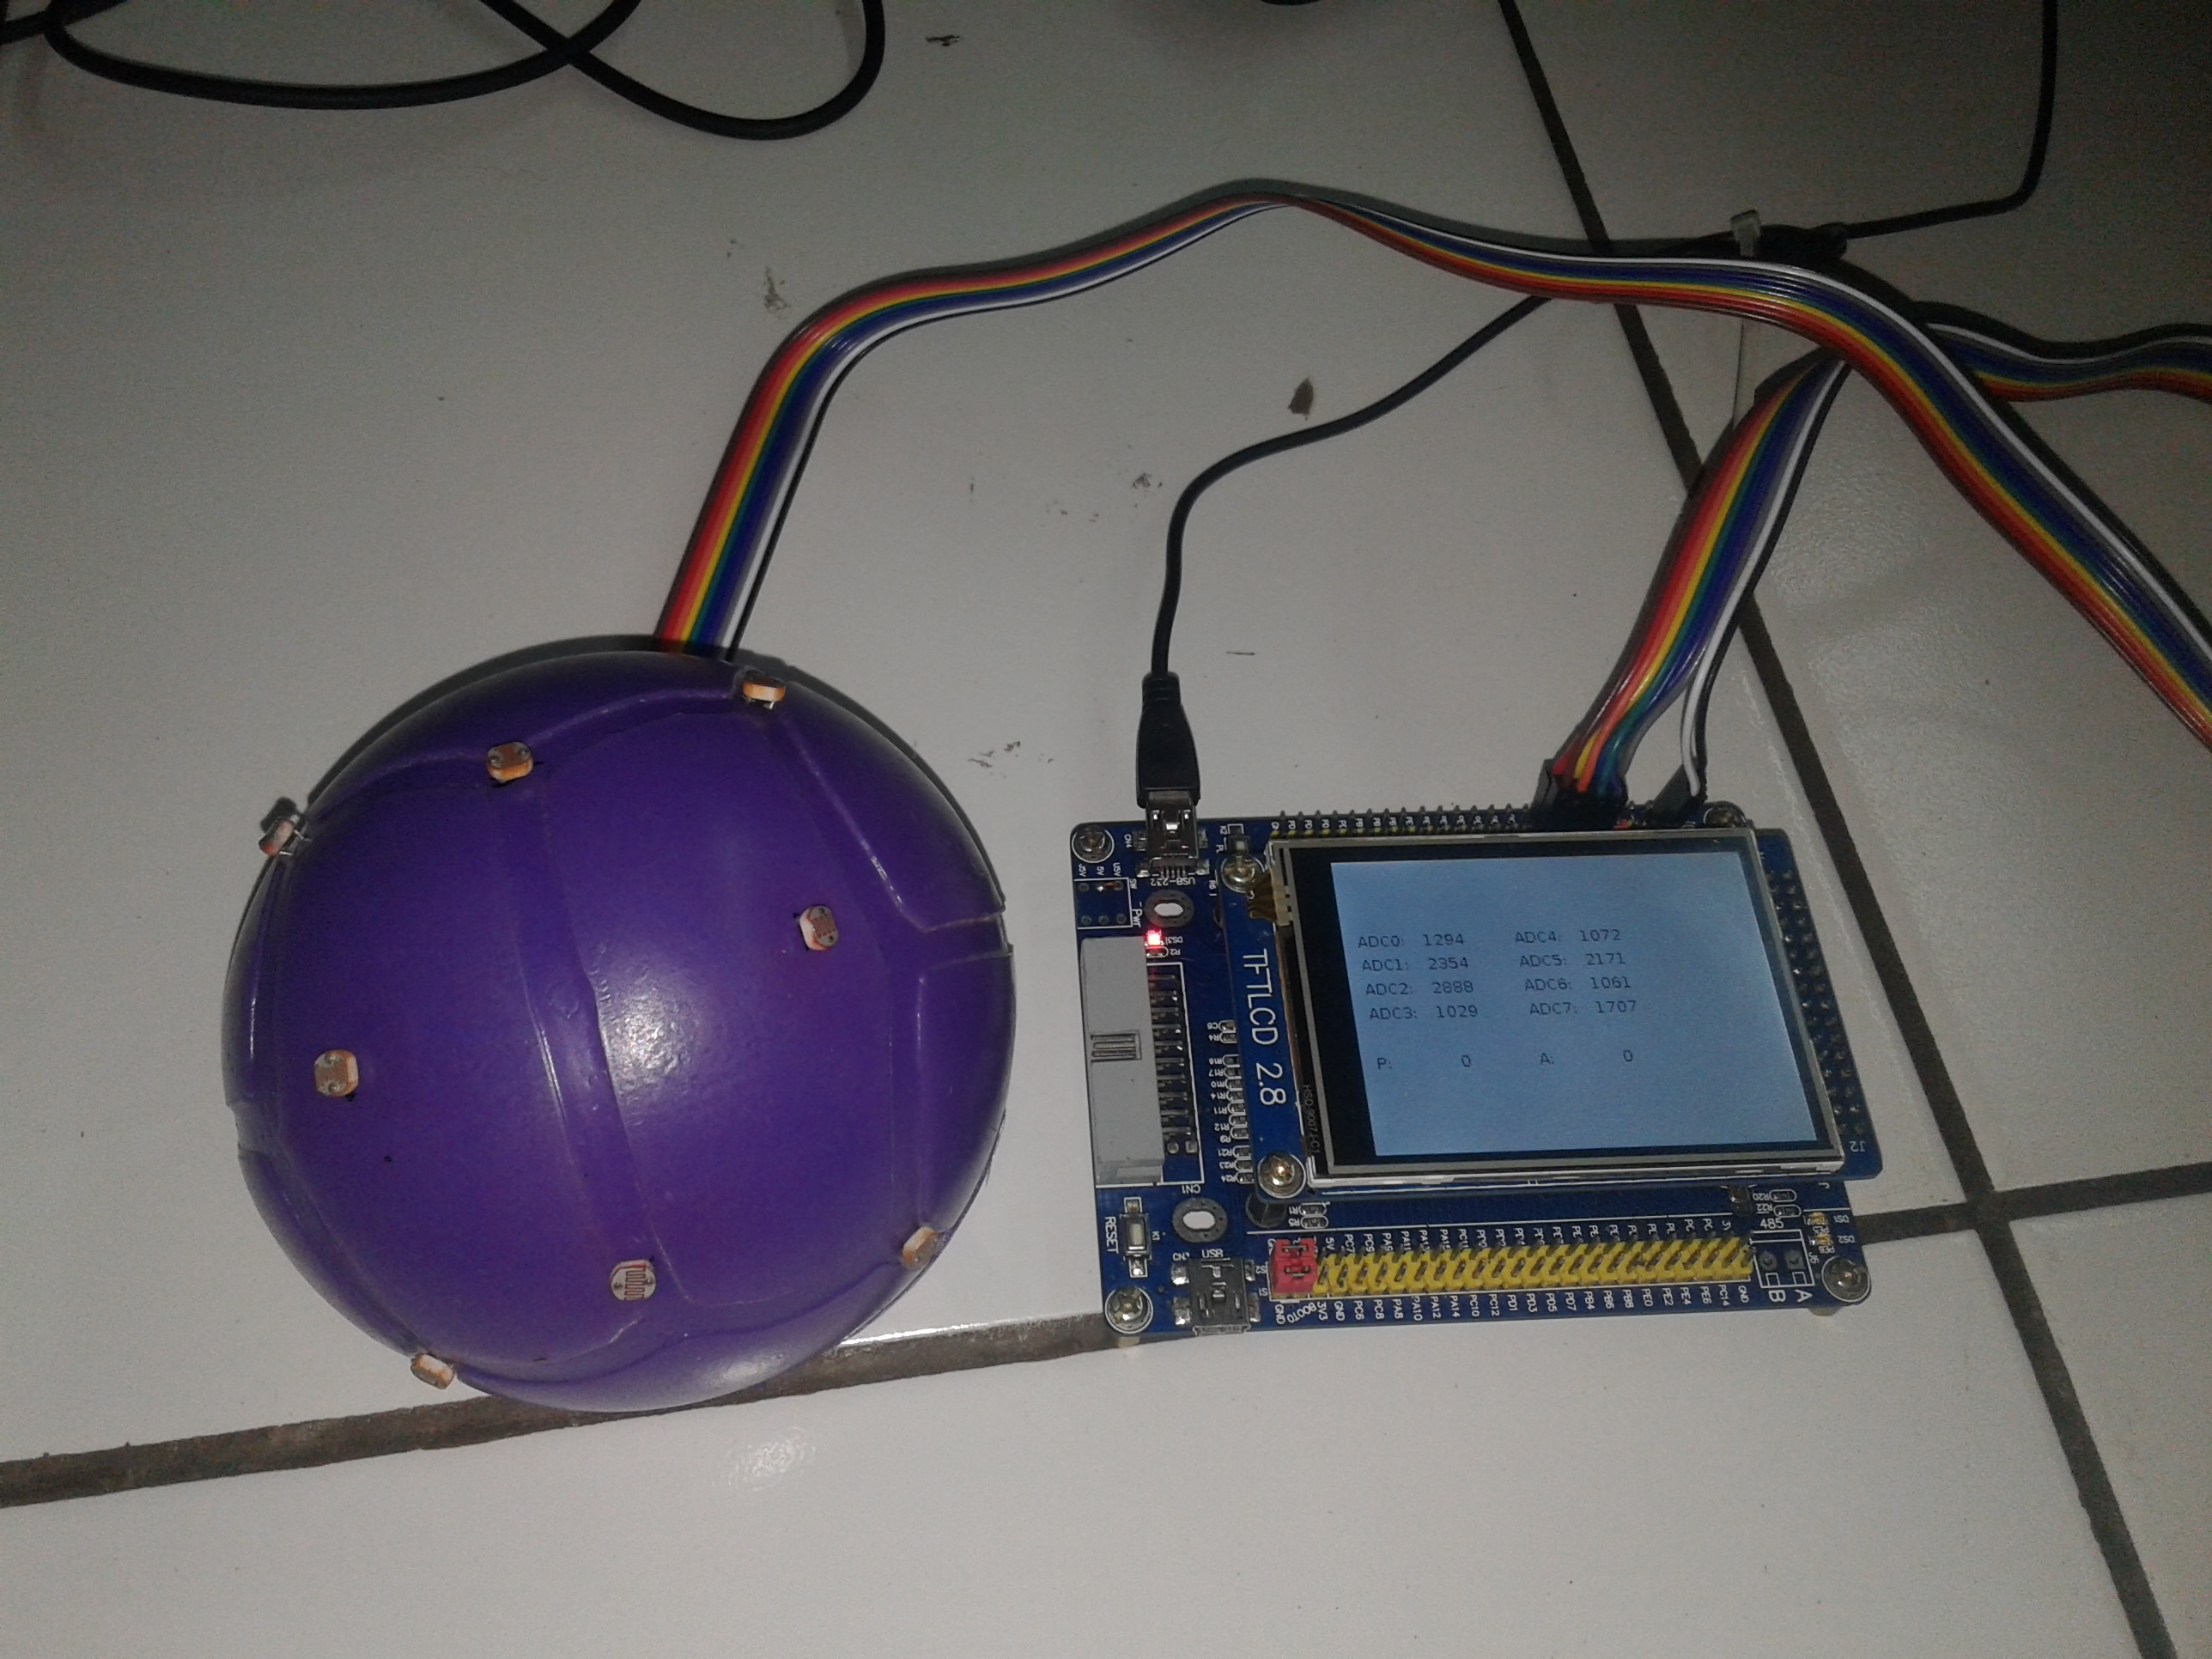
\includegraphics[width=100pt]{wiring}
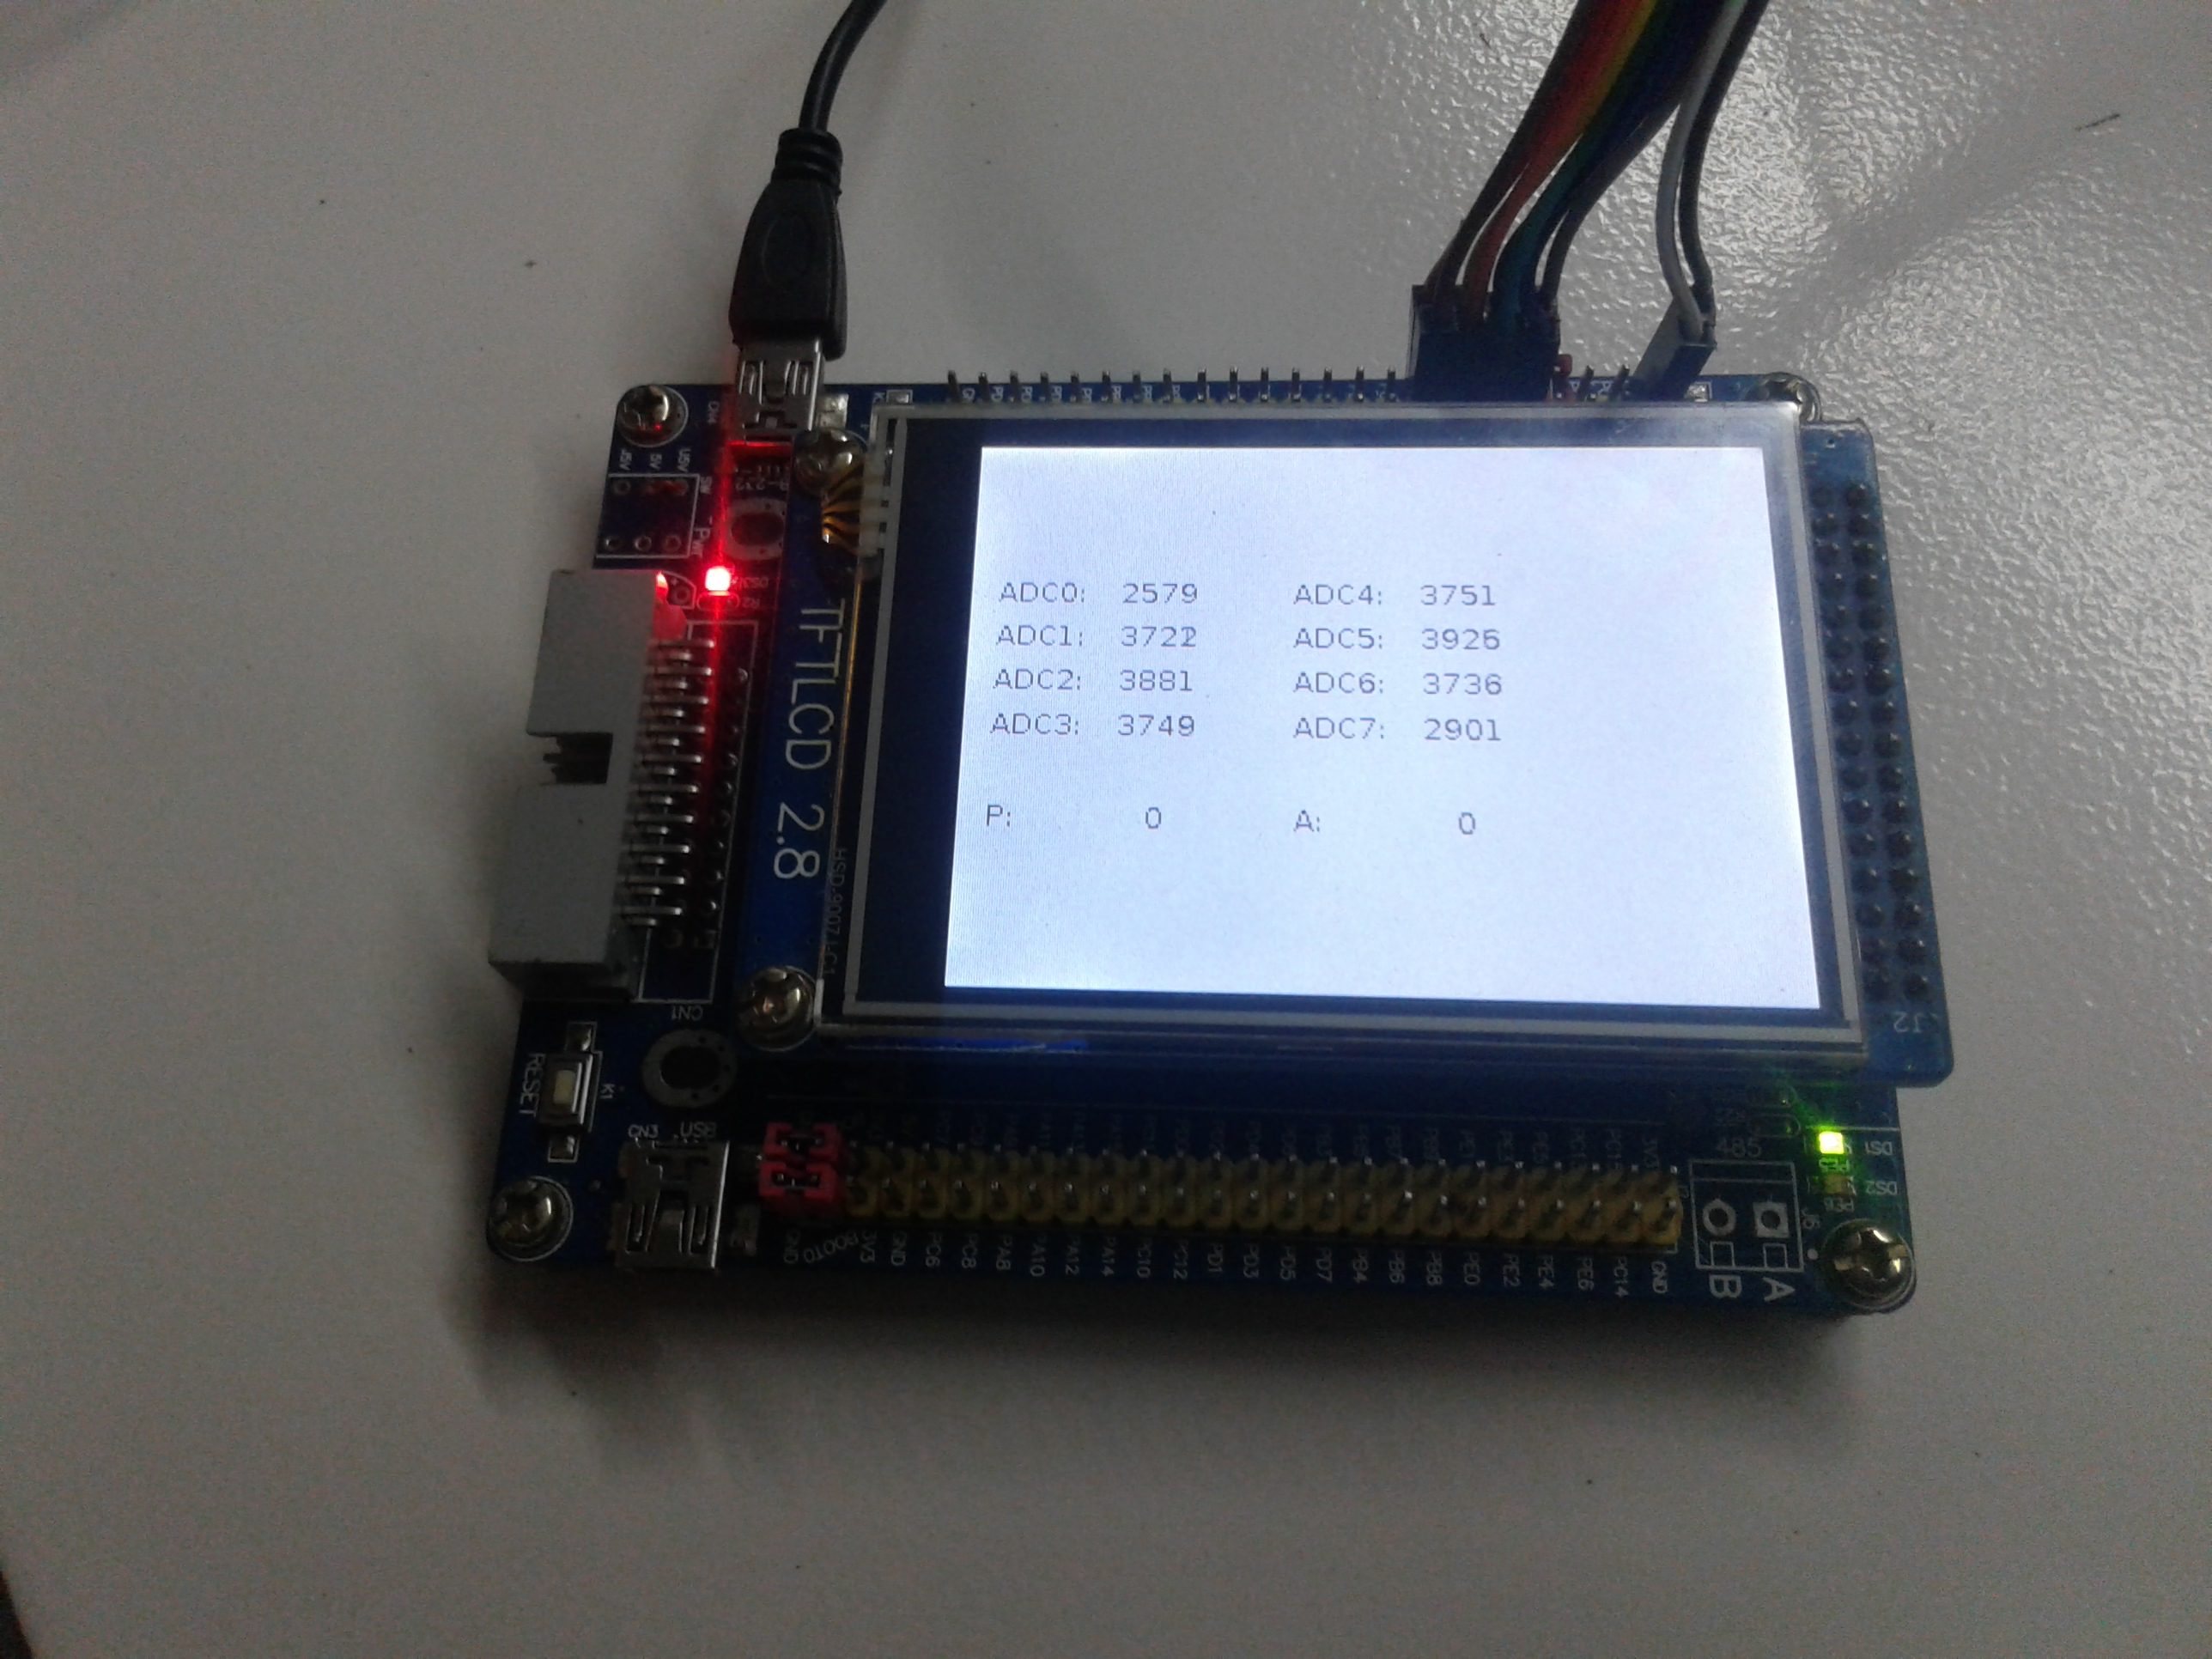
\includegraphics[width=100pt]{interface}

\section{Conclusion}

\section*{Acknowledgment}

\ifCLASSOPTIONcaptionsoff
  \newpage
\fi

\begin{thebibliography}{1}

\bibitem{sensor_array}
Peyman Yousefian, Mohammad Durali, and Mir Abbas Jalali, 
\emph{Optimal Design and Simulation of Sensor Arrays for Solar Motion Estimation},
vol.17, no.6, 2017

\bibitem{sun_sensor_1}
H. Jung and M. L. Psiaki, 
\emph{Tests of magnetometer/sun-sensor orbit determination using flight data},
J. Guid., Control, Dyn., vol. 25, no. 3, pp. 582–590, 2002

\bibitem{sun_sensor_2}
M. L. Psiaki, 
\emph{Autonomous low-earth-orbit determination from magne- tometer and sun sensor data},
J. Guid., Control, Dyn., vol. 22, no. 2, pp. 296–304, 1999

\bibitem{old_sensor_1}
G. Rufino and M. Grassi, 
\emph{Digital sun sensor multi-spot operation},
Sensors, vol. 12, no. 12, pp. 16451–16465, 2012

\bibitem{old_sensor_2}
W.-Y. Li, G.-F. Zhang, Z. You, and F. Xing,
\emph{Error compensation for area digital sun sensor},
Sensors, vol. 12, no. 9, pp. 11798–11810, 2012

\bibitem{old_sensor_3}
K. Ninomiya, Y. Ogawara, K. Tsuno, and S. Akabane,
\emph{High accuracy sun sensor using CCDs},
in Proc. AIAA Guid., Navigat. Control Conf., 1988, pp. 1061–1070

\bibitem{old_sensor_4}
M.-S. Wei, F. Xing, B. Li, and Z. You,
\emph{Investigation of digital sun sensor technology with an N-shaped slit mask},
Sensors, vol. 11, no. 10, pp. 9764–9777, 2011

\end{thebibliography}





\begin{IEEEbiography}[{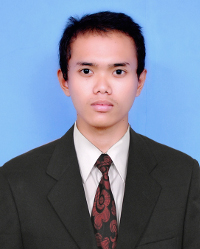
\includegraphics[width=1in,height=1.25in,clip,keepaspectratio]{Foto_Berdasi}}]{Achmadi}
Bachelor from Engineering Physics of Sepuluh Nopember Institute of Technology.
Open-Sources technology entusiast.
Mercenary mid-level technology developer.
\end{IEEEbiography}

\begin{IEEEbiography}[{
\includegraphics[width=1in,height=1.25in,clip,keepaspectratio]{default}}]{Purwadi Agus Darwito}
Lecturer at Engineering Physics of Sepuluh Nopember Institute of Technology.
Control-System technology entusiast.
\end{IEEEbiography}

\end{document}


